\subsubsection[„Josephi“{}-Messe F{}-Dur op. 62]{„Josephi“-Messe F-Dur
op. 62}


Namensgeber der Messe war Högns Hausarzt Dr. Joseph Stern. Als Högn die
„Josephi“-Messe fertig komponiert hatte, bot er Stern bei einem
Arztbesuch mit Verweis auf ihre gute Freundschaft an, der neuen Messen
einen Namen zu geben. Stern bestimmte seinen Namenspatron, den Heiligen
Joseph, als Namenspatron auch für die Messe. Sie trägt deshalb den
Titel: \zitat{„Missa in honorem Sancti Josephi“}.\footnote{
Interview mit Dr. Josephi Stern, 21.2.2003, Absatz 2} Wie aus mehreren
Dokumenten und Interviews hervorgeht, hieß die Messe in Kurzform
„Josephi“-Messe.

\begin{center}
\begin{minipage}{3.884cm}
\begin{flushleft}
\tablefirsthead{}
\tablehead{}
\tabletail{}
\tablelasttail{}
\begin{supertabular}{m{3.684cm}}

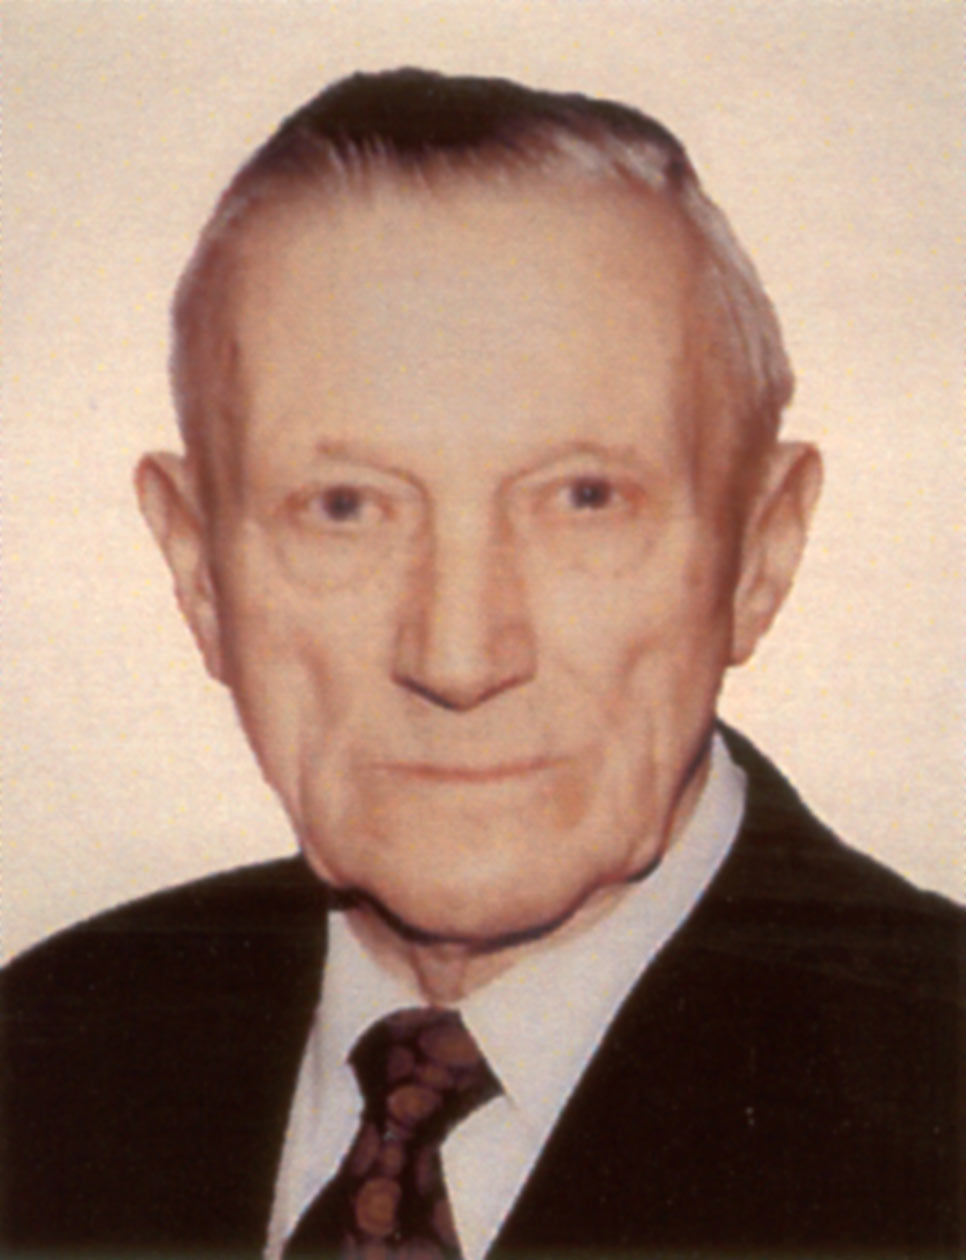
\includegraphics[width=3.501cm,height=4.533cm]{pictures/zulassungsarbeit-img106.jpg}

Dr. Joseph Stern\\
\end{supertabular}
\end{flushleft}
\end{minipage}
\end{center}


\begin{figure}
\img{}
\caption{}
\end{figure}

\subparagraph{Aufführungen}
Eine Reihe von Dokumenten belegt eine rege Aufführungspraxis über
Jahrzehnte hinweg. Die erste uns bekannte Aufführung fand am 14.6.1953
zur Installation des neuen Pfarrers Franz Seraph Reicheneder statt. Ein
Zeitungsartikel bescheinigte dem \zitat{„klangvollen Chor“}
unter der Leitung des Komponisten den \zitat{„ergreifenden“}
Vortrag der \zitat{„Missa St. Josephi.“ } \footnote{Dokument
Nr. 41, Zeitungsartikel aus dem Viechtacher Bayerwald-Boten, 15.6.1953}

Wie es zu der Aufführung der „Josephi“-Messe in der Kirche St. Magdalena
in Plattling am 19.3.1957 gekommen war, ist nicht bekannt. In einer
Ankündigung am Tag der Aufführung in der Plattlinger Zeitung wird Högns
\zitat{„romantisch, liebenswerter Kompositionsstil“
} \footnote{Dokument Nr. 43, Zeitungsartikel aus der Plattlinger
Zeitung, 19.3.1957} gelobt. Weiter heißt es: \zitat{„Das
Benediktus für Sopransolo und Chor wird sicher allen gefallen, die die
Musik nicht erst über den Verstand, sondern gleich ins Herz fließen
lassen wollen.“ } \footnote{Dokument Nr. 43, Zeitungsartikel aus der
Plattlinger Zeitung, 19.3.1957} Auf einer Postkarte bedankte sich der
Chorleiter Gustl Gudmer bei Högn für das Ausleihen des Notenmaterials
der „Josephi-Messe“ und versicherte ihm: \zitat{„Sie }(die
„Josephi“-Messe)\zitat{ hat am Josephsfest gut gefallen. Ich
habe verschiedene Stimmen darüber gehört. Unserer geistlicher Rat hier
hat sich sehr gefreut über die Aufführung.“ } \footnote{Dokument Nr.
44, Brief von Gustl Gudmer an August Högn, 22.3.1957}

Dem Engagement von Högns ehemaliger Chorsängerin Maria Schröck ist es zu
verdanken, dass die „Josephi“-Messe am 19.3.1959 in Deggendorf vom Chor
an St. Martin aufgeführt wurde. \footnote{Interview Nr. 4, Maria
Schröck, 30.12.2002, Absatz 28} Maria Schröck, die 1950 nach Deggendorf
geheiratet hatte und seitdem Mitglied im Kirchenchor St. Martin war,
machte ihrem Chorregenten Fritz Goller, dem Neffen von Vinzenz Goller,
den Vorschlag, eine Messe von August Högn einzustudieren. Goller ging
auf diesen Vorschlag anfangs nicht ein. Erst als Maria Schröck ihm
drohte, an Stelle von St. Martin ein Aufführung der „Josephi“-Messe in
der Pfarrkirche Mariä Himmelfahrt anzustreben – es herrschte eine
gewisse Rivalität zwischen den Kirchenmusiken von St. Martin und Mariä
Himmelfahrt – ging Goller auf ihr Anliegen ein. Auf einer
Faschingsfeier des Kirchenchores trug Fritz Goller folgendes Gedicht
vor, das Bezug auf die unbeirrbare Vorgehensweise von Maria Schröck
nimmt:

\zitat{Die Schröck Maria eine Messe bringt, }

\begin{center}
\begin{minipage}{4.598cm}
\begin{flushleft}
\tablefirsthead{}
\tablehead{}
\tabletail{}
\tablelasttail{}
\begin{supertabular}{m{4.3980002cm}}

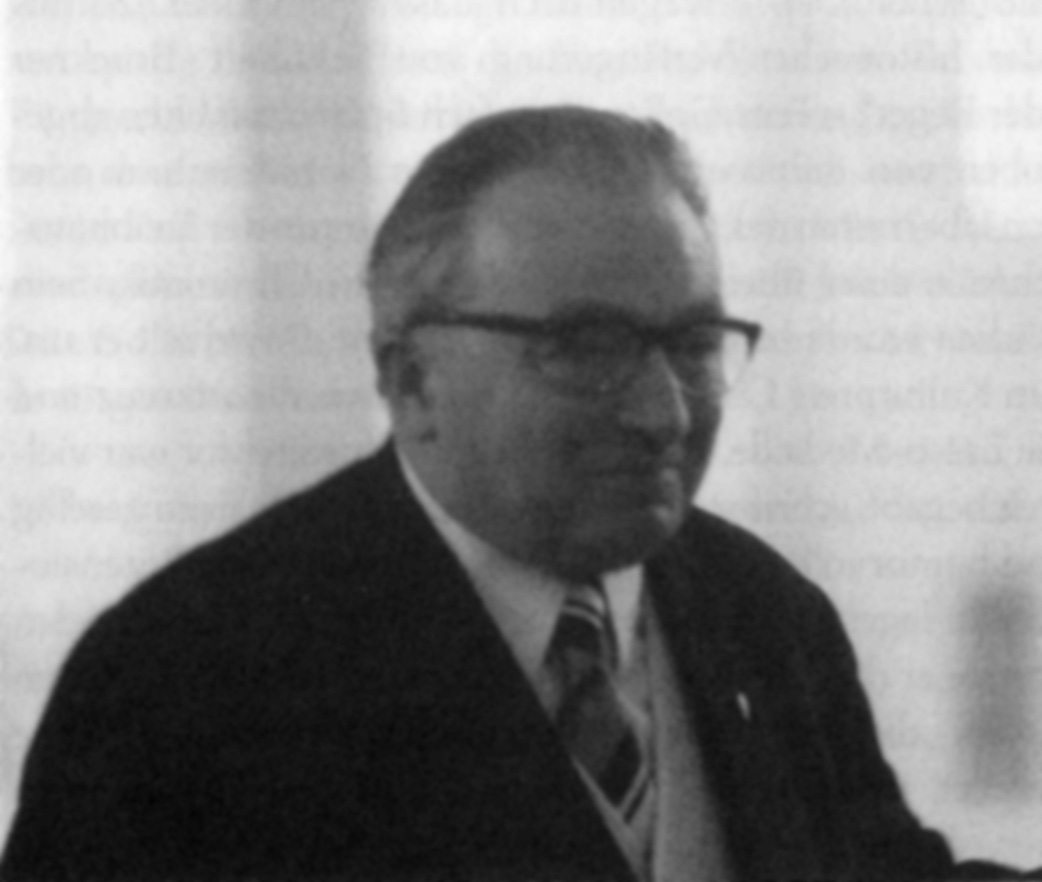
\includegraphics[width=4.216cm,height=3.577cm]{pictures/zulassungsarbeit-img107.jpg}

Fritz Goller \\
\end{supertabular}
\end{flushleft}
\end{minipage}
\end{center}


\begin{figure}
\img{}
\caption{}
\end{figure}

\zitat{und um ihre Aufführung ringt.}

\zitat{Sie nimmt die Messe unterm Arm}

\zitat{und sagt zum Chorregent brühwarm:}

\zitat{„Die Messe trag ich jetzt nach Himmelfahrt rein,}

\zitat{da wird dann bald die Aufführung sein.“ }\footnote{
Interview Nr. 4, Maria Schröck, 30.12.2002, Absatz 42}

Zur „Josephi“-Messe äußerte sich Fritz Goller in einem Zeitungsartikel,
der einen Tag vor der Aufführung erschien:\zitat{ }Die
Messe\zitat{ „verrät gediegene Handwerkskunst, die sich in
einer sauberen satztechnischen Handschrift äußert, Sinn für harmonische
Farbigkeit hat, ohne in spätromantische Chromatik abzugleiten, und sich
der Mittel des Kontrastes in der Gegenüberstellung kraftvoller Unisoni
und motivisch aufgelockerter Chorsätze bedient.“ } \footnote{Dokument
Nr. 42, Zeitungsartikel aus der Deggendorfer Zeitung, 18.3.1959} August
Högn war bei der Aufführung in Deggendorf anwesend. Man gratulierte ihm
nach der Messe zu seiner Komposition. Er reagierte aber bescheiden und
trat bald den Nachhauseweg an. \footnote{Interview Nr. 4, Maria
Schröck, 30.12.2002, Abschnitt 44}

Beim Pfarrerwechsel in Ruhmannsfelden 1974 kam die „Josephi“-Messe
zweimal zum Einsatz. Sie erklang vom Ruhmannsfeldener Kirchenchor unter
der Leitung von Karl Geiger gesungen zur Verabschiedung des alten
Pfarrers Reicheneder am 4.8.1974 \footnote{Dokument Nr. 45,
Zeitungsartikel aus dem Viechtacher Bayerwald-Boten, 6.8.1974, Dokument
Nr. 46, Zeitungsartikel aus dem Regensburger Bistumsblatt, 24.8.1974}
und zur Installation des neuen Pfarrers Otto Krottenthaler am
29.9.1974. \footnote{Dokument Nr. 47, Zeitungsartikel aus dem
Viechtacher Bayerwald-Boten, 4.10.1974}

Weitere Aufführungen der „Josephi“-Messe in Altötting könnten von Högns
Tochter Elfriede Schlumprecht veranlasst worden sein. An Einzelheiten
über die Aufführungen konnte sich Högns Enkelin Gertraud von Molo nicht
erinnern. \footnote{Interview Nr. 20, Gertraud von Molo, 23.11.2004}

\clearpage\subparagraph{Wiederkehrendes Soggetto}
Die einzelnen Teile der „Josephi“-Messe (siehe Band III, Seite 33 – 67)
werden durch ein in fast alle Sätzen auftretendes Soggetto thematisch
zusammengehalten. Diese Technik ist Högn sicherlich in den Messen von
Vinzenz Goller begegnet. In der Missa in honorem St. Stefani
Protomatyris op. 8 arbeitete Goller besonders streng mit
wiederkehrenden Soggetti. Das Soggetto wird in der „Josephi“-Messe
schon im Orgelvorspiel des im 4/4-Takt stehenden Kyries angedeutet und
im Takt 9 zum ersten Mal vom Chor gesungen. Das aus vier Tönen
bestehende Soggetto beginnt auf dem Quintton der Tonika und gelangt
über den Terzton der Tonika und den Leitton der F-Dur-Tonleiter zum
Grundton. Indem Högn unmittelbar vor Erreichen des Grundtons den
Leittons auf der betonten dritten Zählzeit setzt und den Leitton
darüber hinaus dominantisch harmonisiert (Takt 9), erhält das Soggetto
bei dieser Note eine Betonung, als eine Betonung zur Taktmitte hin. Der
Beginn des Soggettos auf der Quinte der Tonika, also auf dem „schwachen
Vertreter“ der Tonika, suggeriert einen unbetonten Einstieg ins
Soggetto, sodass die Betonung zur Taktmitte verstärkter wahrgenommen
wird. Diese sich aus der Struktur des Soggettos ergebende
Artikulationsweise verleiht der gleichmäßigen Viertelbewegung des
Soggettos einen schwungvollen 2er Puls. Nicht nur das Kyrie, in dem das
Soggetto am meisten verarbeitet wird, sondern auch alle anderen
Messteile, in denen es vorkommt, scheinen den „Schwung“ des Soggettos
anzunehmen, sodass die ganze Messe vom schwingenden Puls des Soggettos
durchdrungen zu sein scheint.

\begin{center}
\begin{minipage}{4.736cm}
\begin{flushleft}
\tablefirsthead{}
\tablehead{}
\tabletail{}
\tablelasttail{}
\begin{supertabular}{m{4.5360003cm}}

\begin{figure}
\img{}
\caption{}
\end{figure}

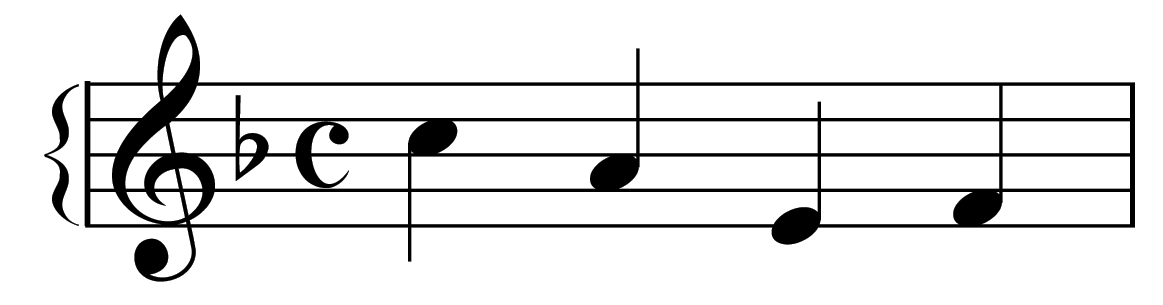
\includegraphics[width=4.307cm,height=1.233cm]{pictures/zulassungsarbeit-img108.png}

Soggetto der „Josephi“-Messe\\
\end{supertabular}
\end{flushleft}
\end{minipage}
\end{center}
\begin{flushleft}
\tablefirsthead{}
\tablehead{}
\tabletail{}
\tablelasttail{}
\begin{supertabular}{m{8.196cm}m{7.783cm}}

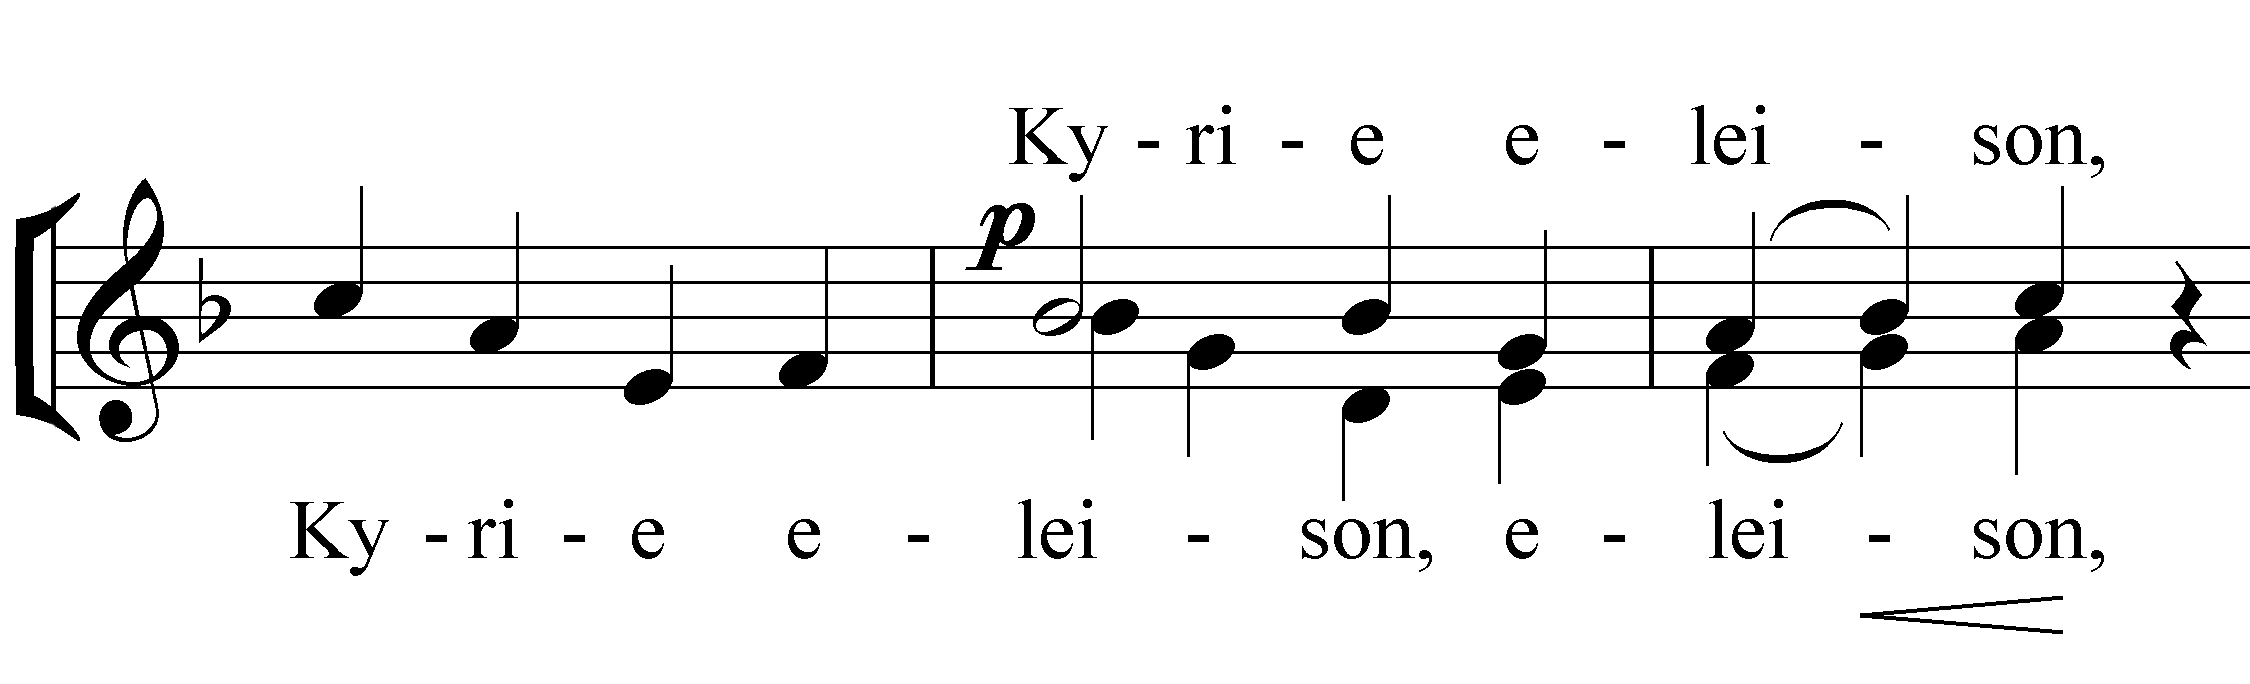
\includegraphics[width=7.678cm,height=2.325cm]{pictures/zulassungsarbeit-img109.png}

\begin{figure}
\img{}
\caption{}
\end{figure}

Kyrie, Takt 9 – 11, Sopran und Alt &

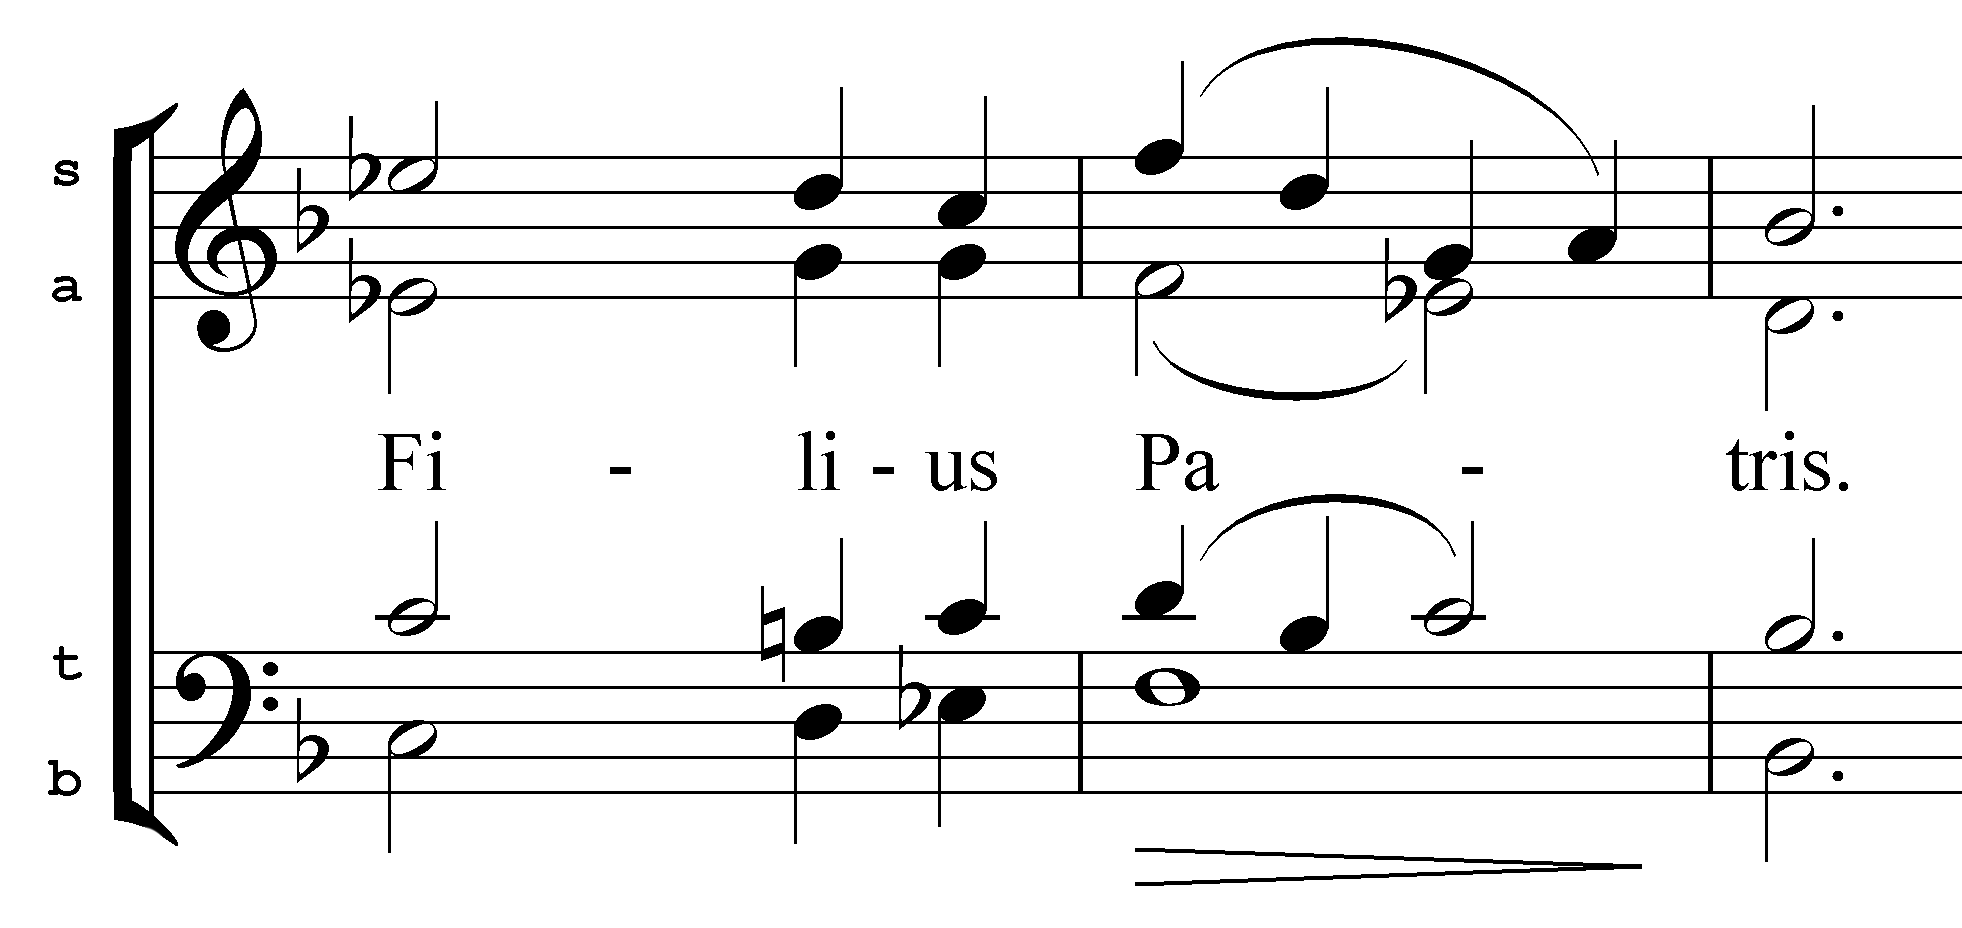
\includegraphics[width=6.592cm,height=3.339cm]{pictures/zulassungsarbeit-img110.png}

Gloria, Takt 28 – 30, Chor\\
\end{supertabular}
\end{flushleft}
\begin{flushleft}
\tablefirsthead{}
\tablehead{}
\tabletail{}
\tablelasttail{}
\begin{supertabular}{m{8.281cm}m{7.6990004cm}}

\begin{figure}
\img{}
\caption{}
\end{figure}

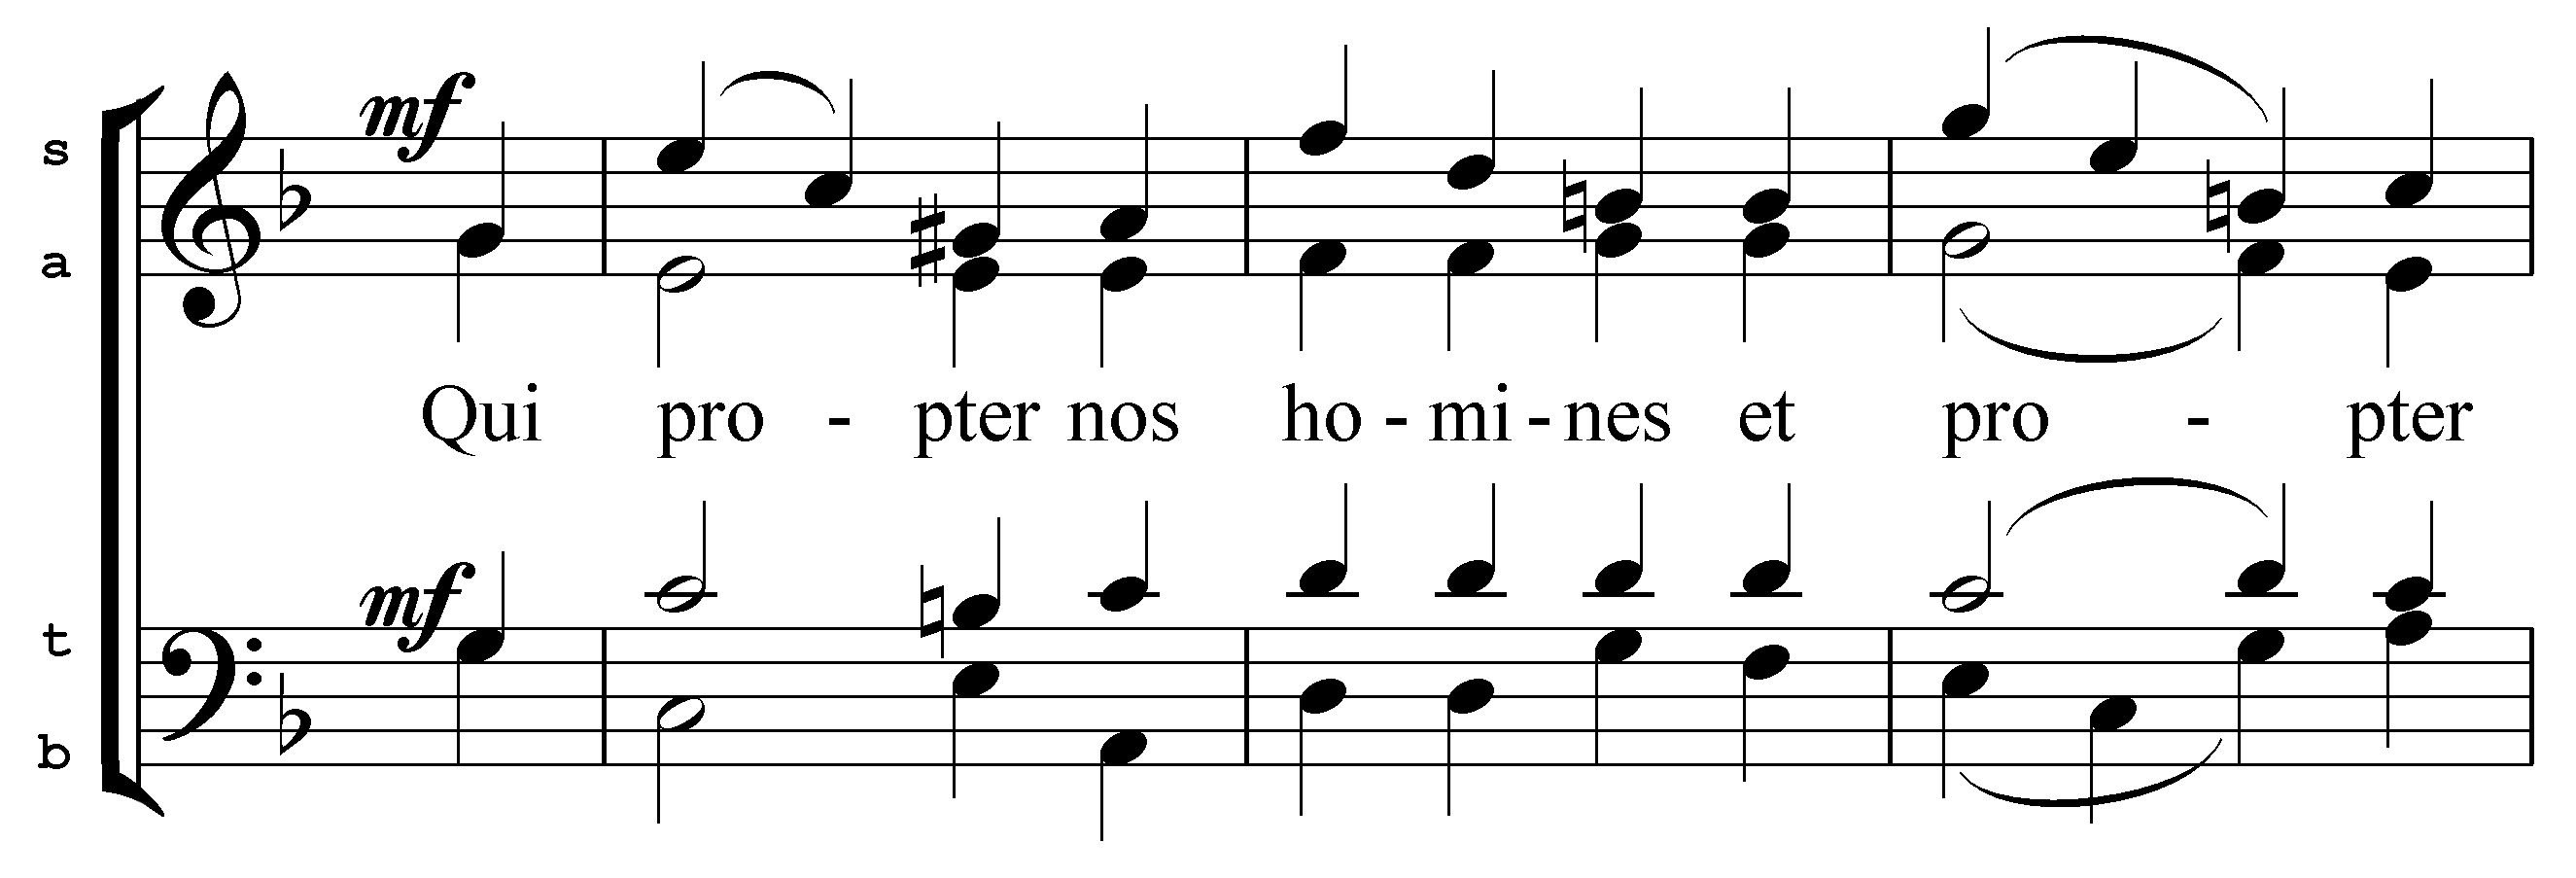
\includegraphics[width=8.098cm,height=3.069cm]{pictures/zulassungsarbeit-img111.png}

Credo, Takt 36 – 39, Chor &

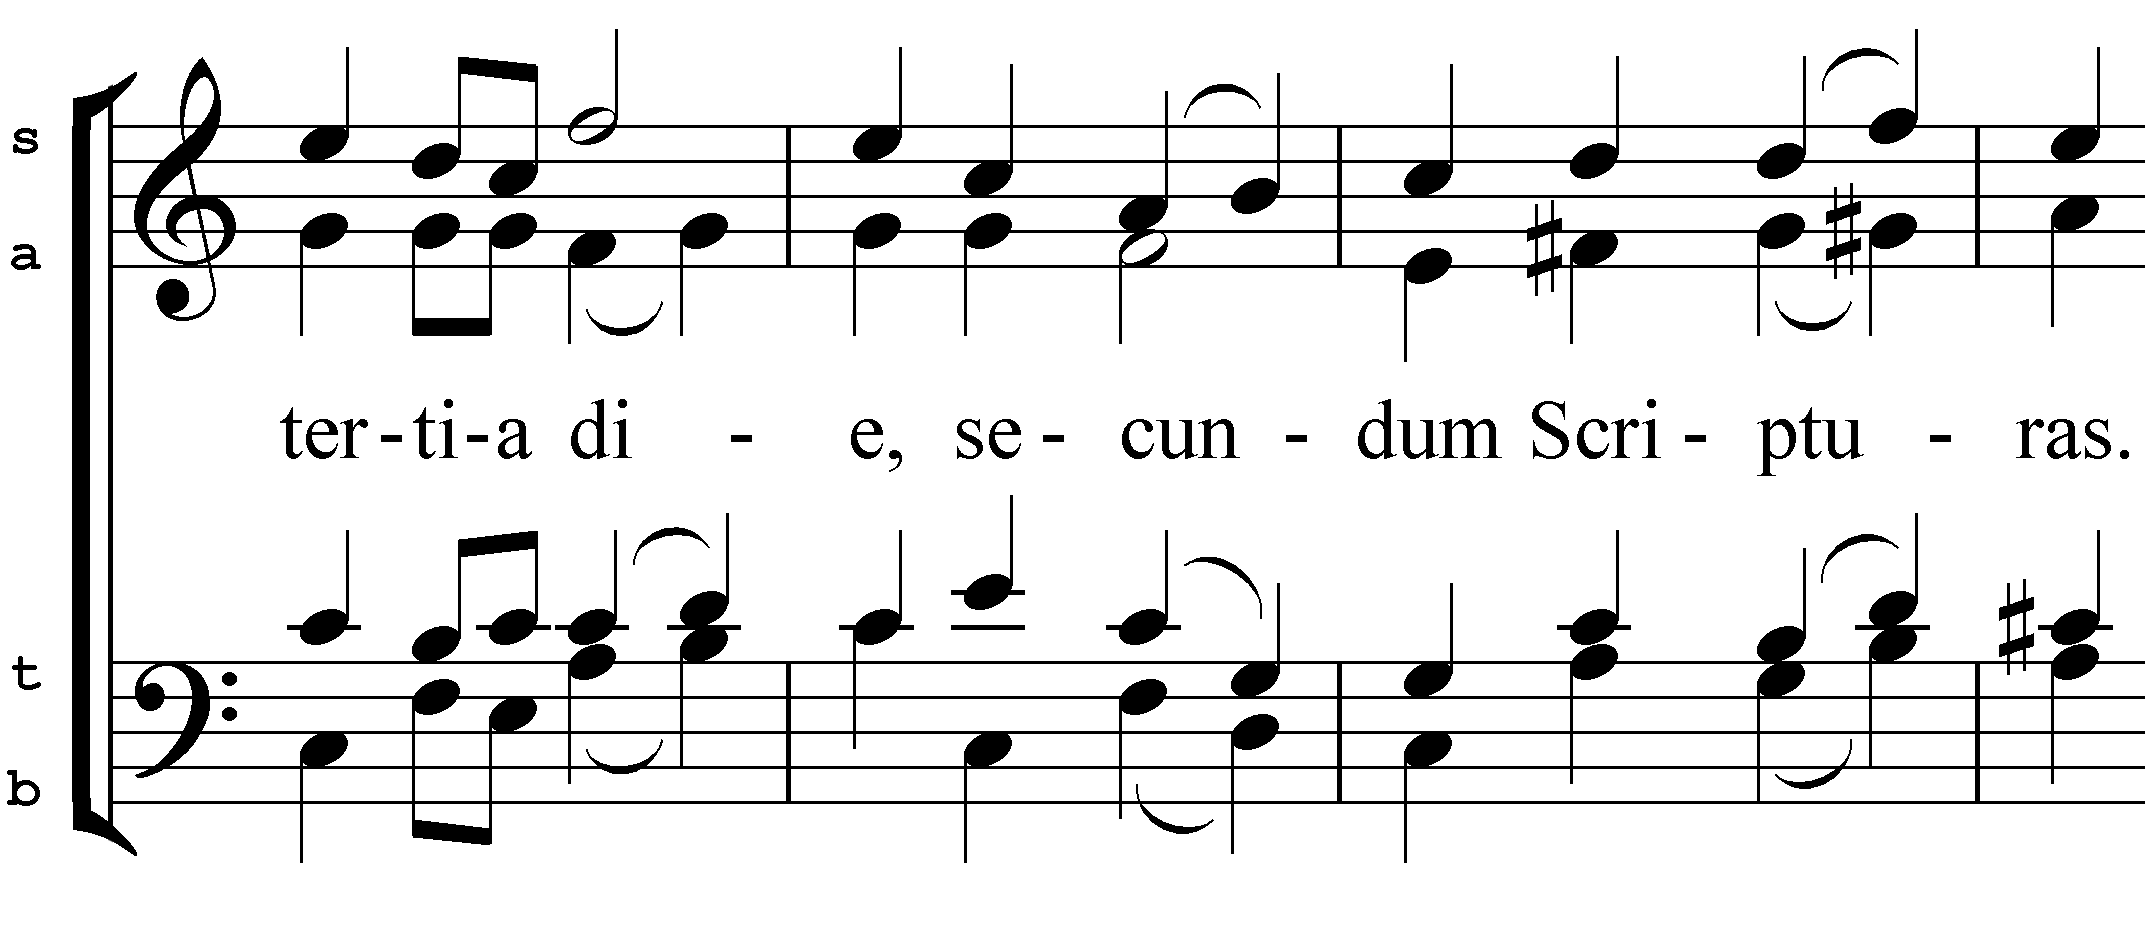
\includegraphics[width=7.207cm,height=3.216cm]{pictures/zulassungsarbeit-img112.png}
\begin{figure}
\img{}
\caption{}
\end{figure}
Credo, Takt 69 – 72, Chor\\
\end{supertabular}
\end{flushleft}
\begin{flushleft}
\tablefirsthead{}
\tablehead{}
\tabletail{}
\tablelasttail{}
\begin{supertabular}{m{8.778cm}m{6.208cm}}
\begin{figure}
\img{}
\caption{}
\end{figure}
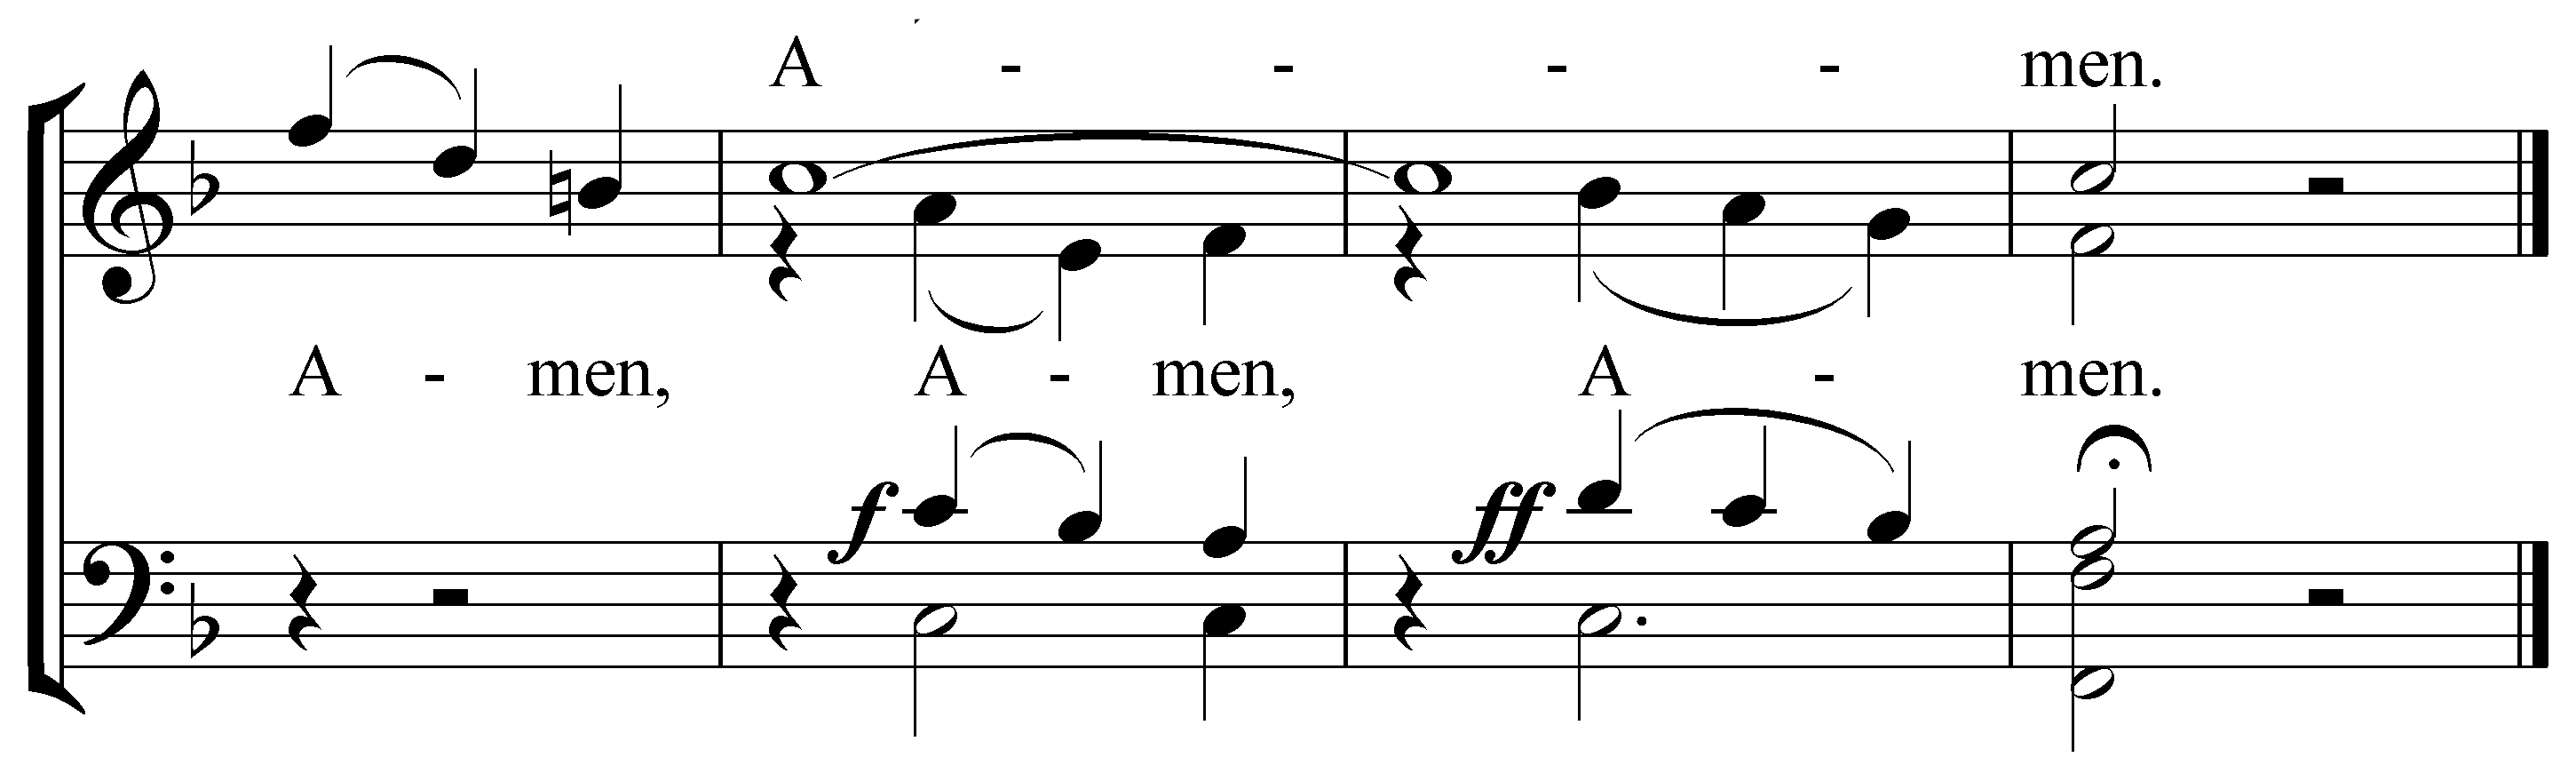
\includegraphics[width=8.595cm,height=2.515cm]{pictures/zulassungsarbeit-img113.png}

Credo, Takt 133 – 136, Chor &
\begin{figure}
\img{}
\caption{}
\end{figure}
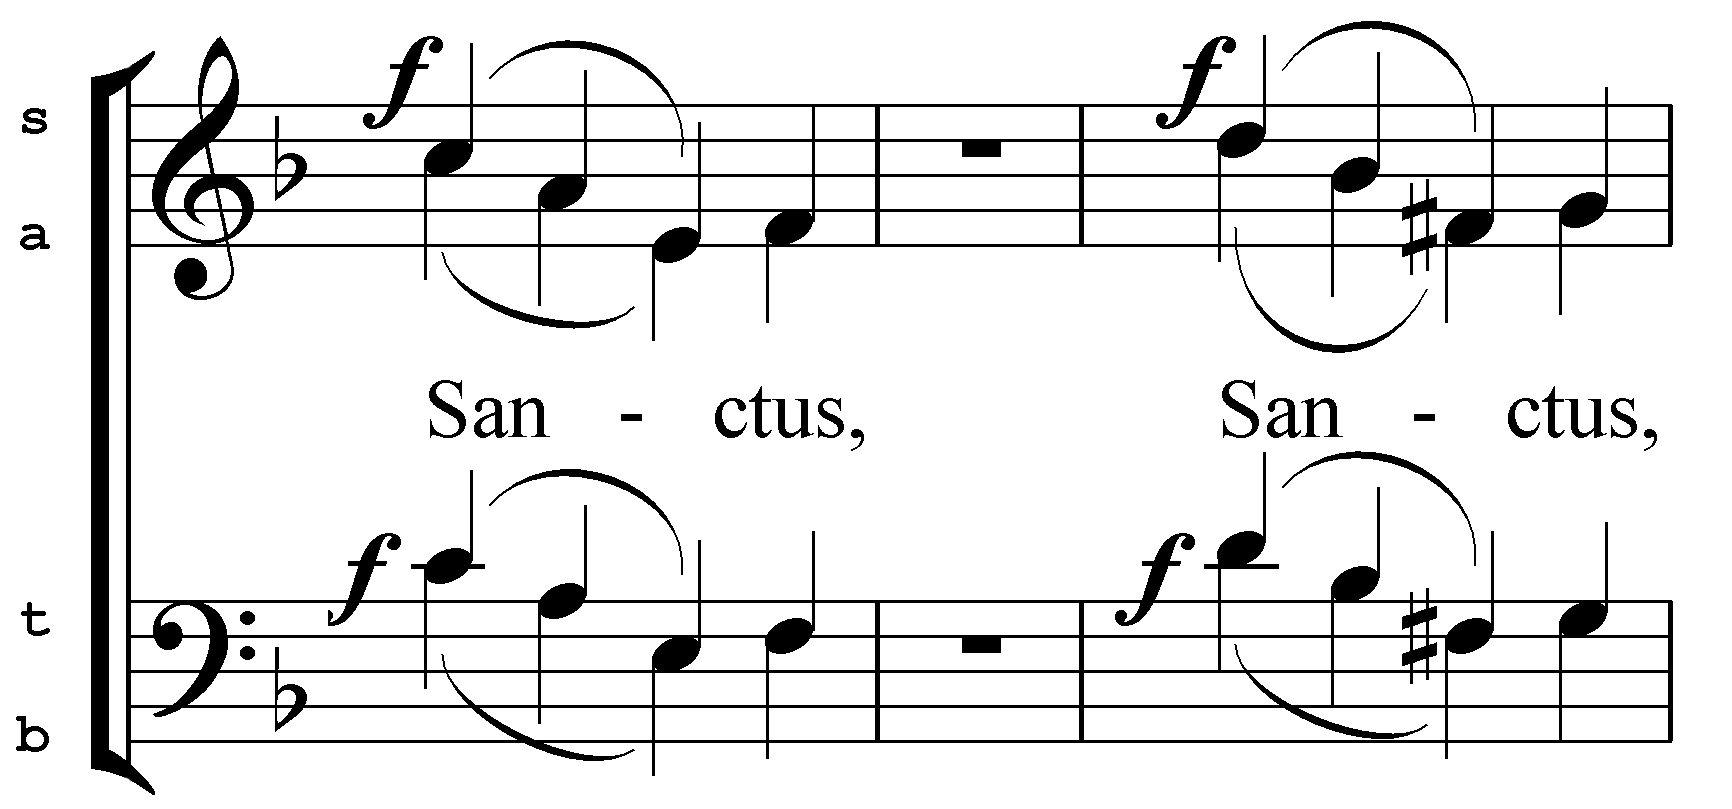
\includegraphics[width=5.681cm,height=2.76cm]{pictures/zulassungsarbeit-img114.png}

Sanctus, Takt 3 – 5, Chor\\
\end{supertabular}
\end{flushleft}
\begin{flushleft}
\tablefirsthead{}
\tablehead{}
\tabletail{}
\tablelasttail{}
\begin{supertabular}{m{7.676cm}m{6.372cm}}
\begin{figure}
\img{}
\caption{}
\end{figure}
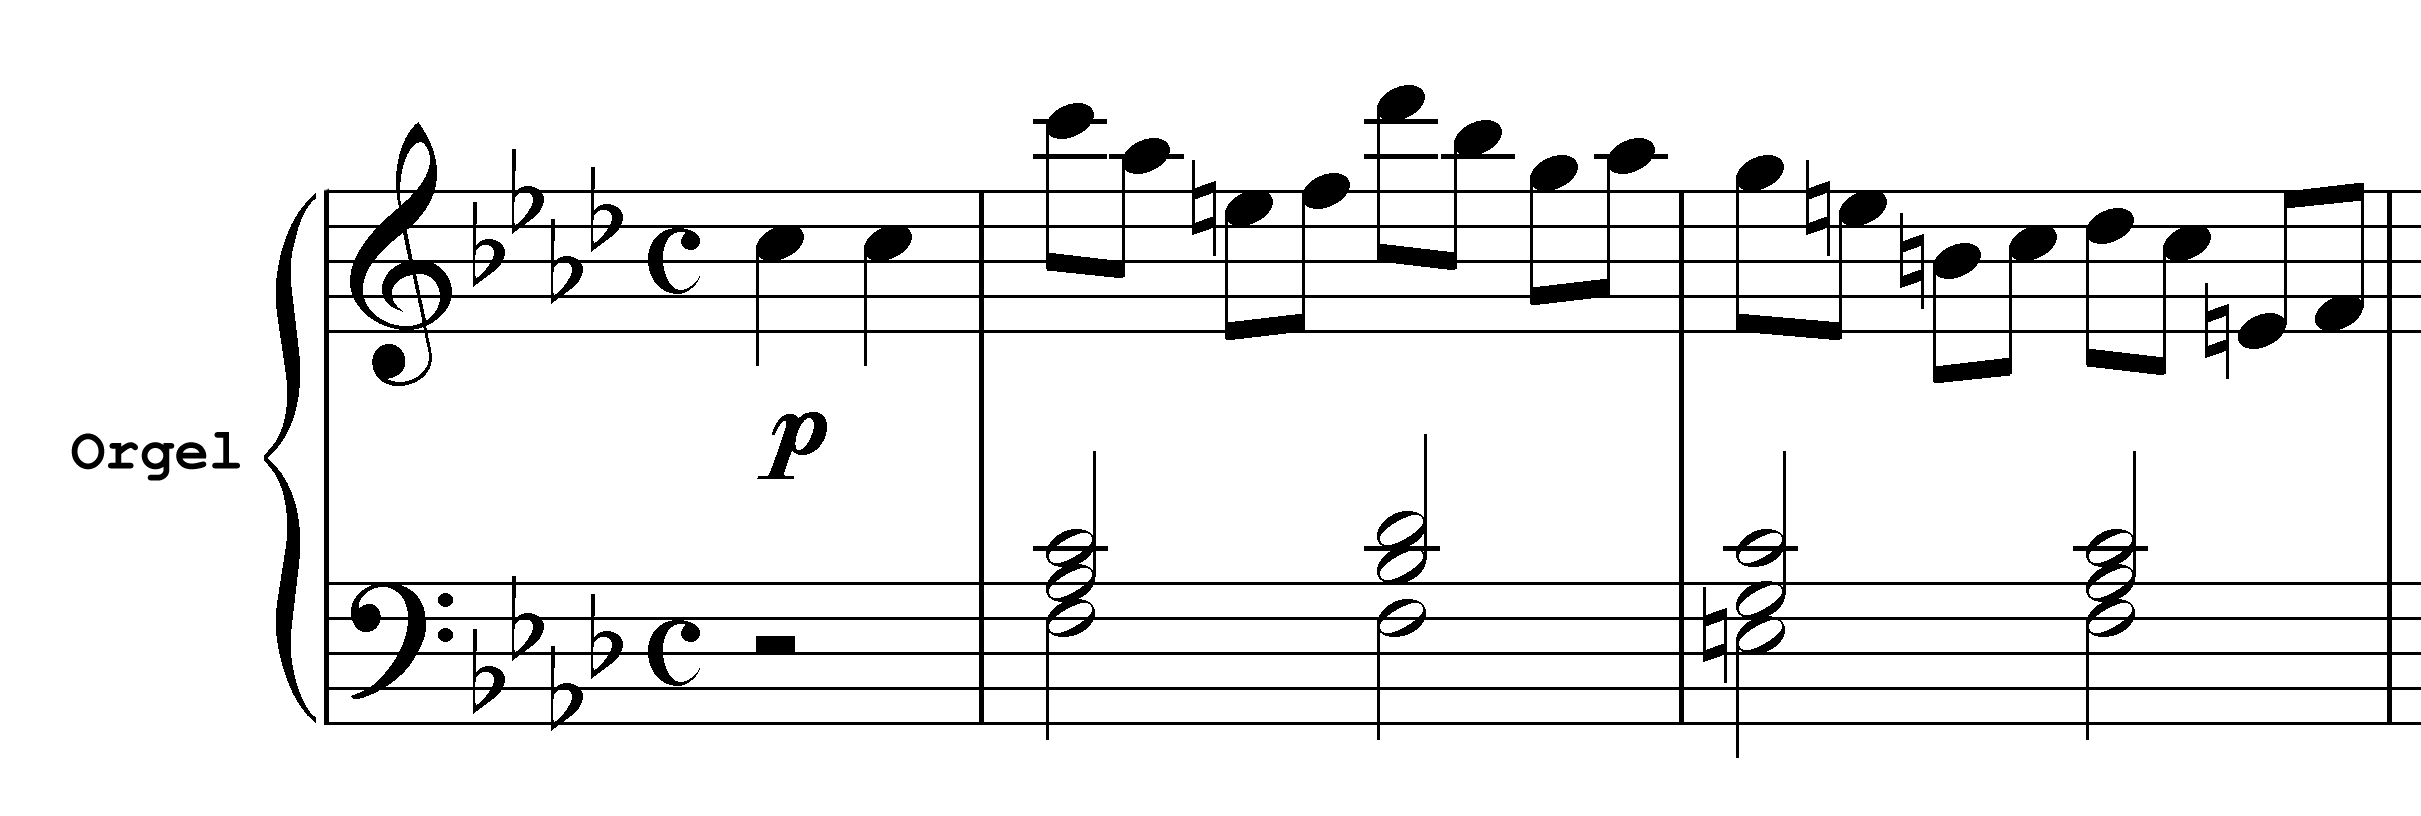
\includegraphics[width=7.493cm,height=2.828cm]{pictures/zulassungsarbeit-img115.png}

Agnus Dei, Takt 1 – 3, Orgel &
\begin{figure}
\img{}
\caption{}
\end{figure}
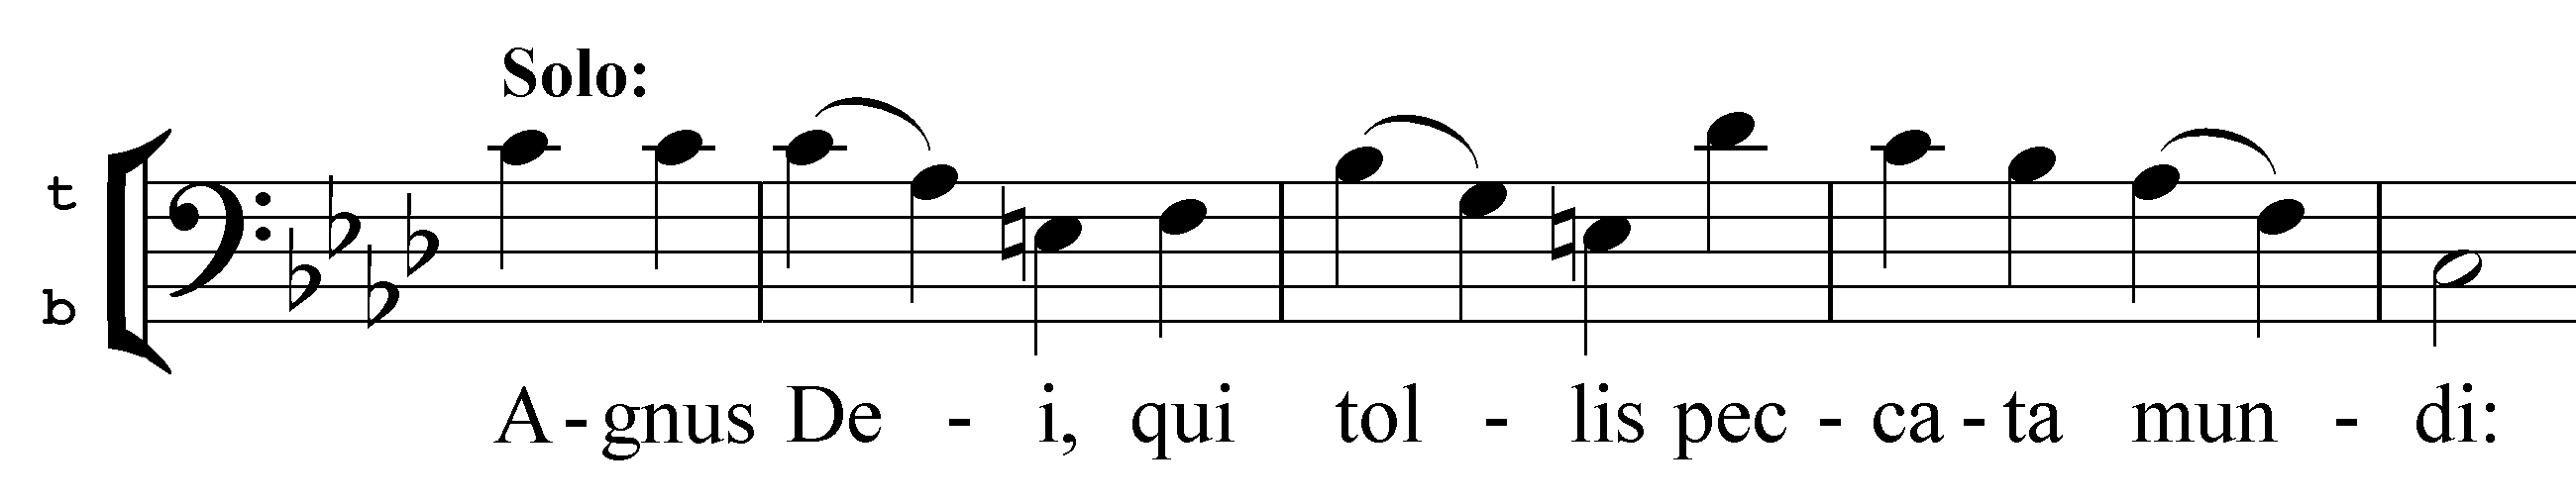
\includegraphics[width=6.018cm,height=1.85cm]{pictures/zulassungsarbeit-img116.png}
\begin{figure}
\img{}
\caption{}
\end{figure}
Agnus Dei, Takt 5 – 9, Bass-Solo\\
\end{supertabular}
\end{flushleft}
\begin{flushleft}
\tablefirsthead{}
\tablehead{}
\tabletail{}
\tablelasttail{}
\begin{supertabular}{m{5.3650002cm}m{5.875cm}}

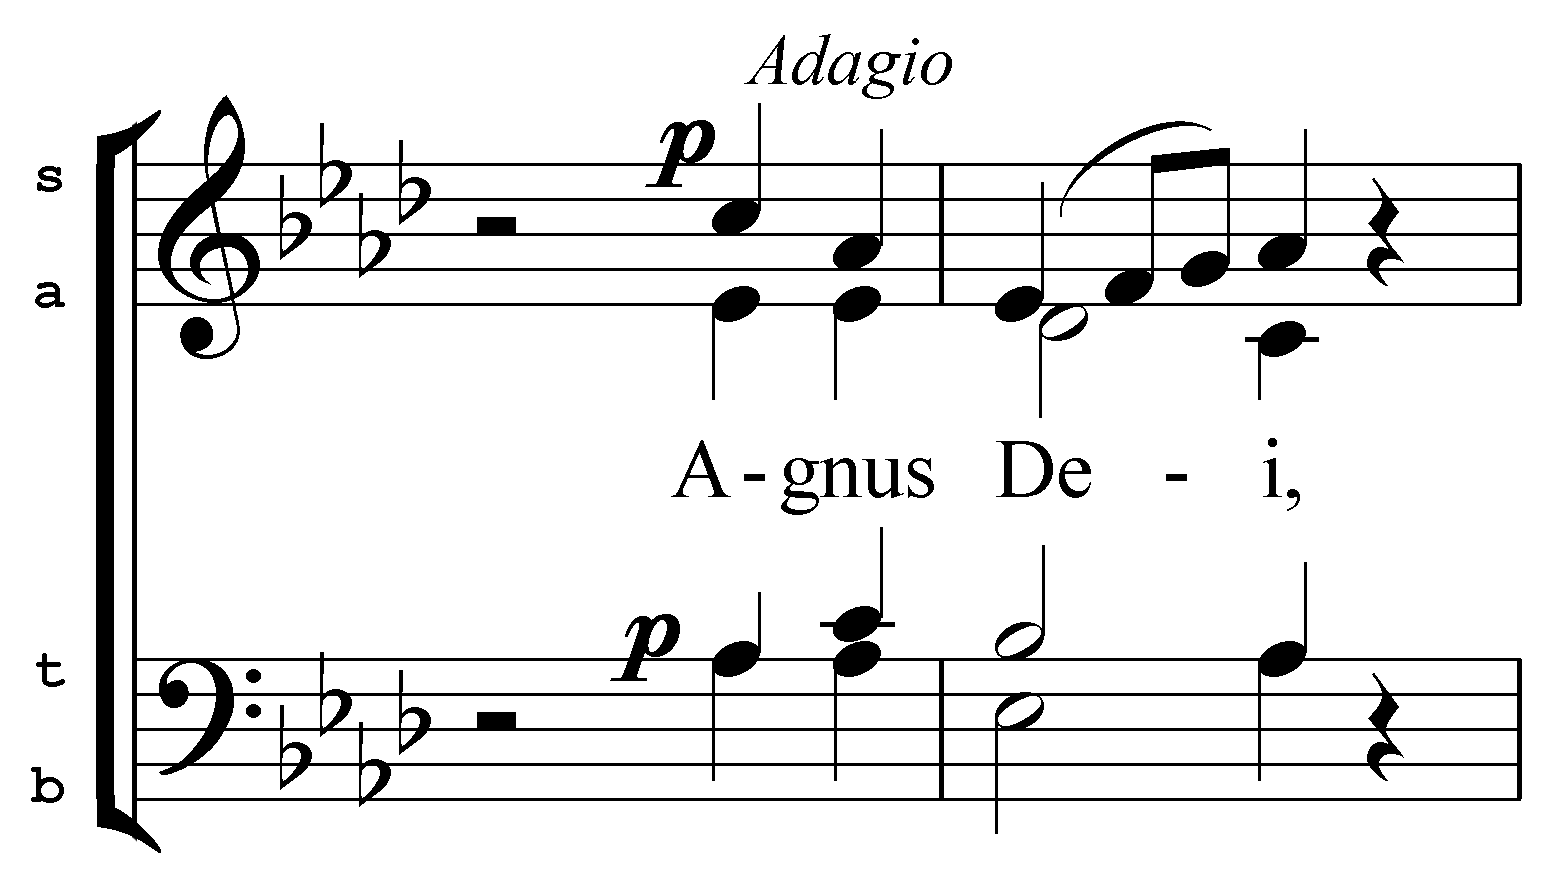
\includegraphics[width=5.182cm,height=3.087cm]{pictures/zulassungsarbeit-img117.png}
\begin{figure}
\img{}
\caption{}
\end{figure}
Agnus Dei, Takt 33 – 34, Chor &
\begin{figure}
\img{}
\caption{}
\end{figure}
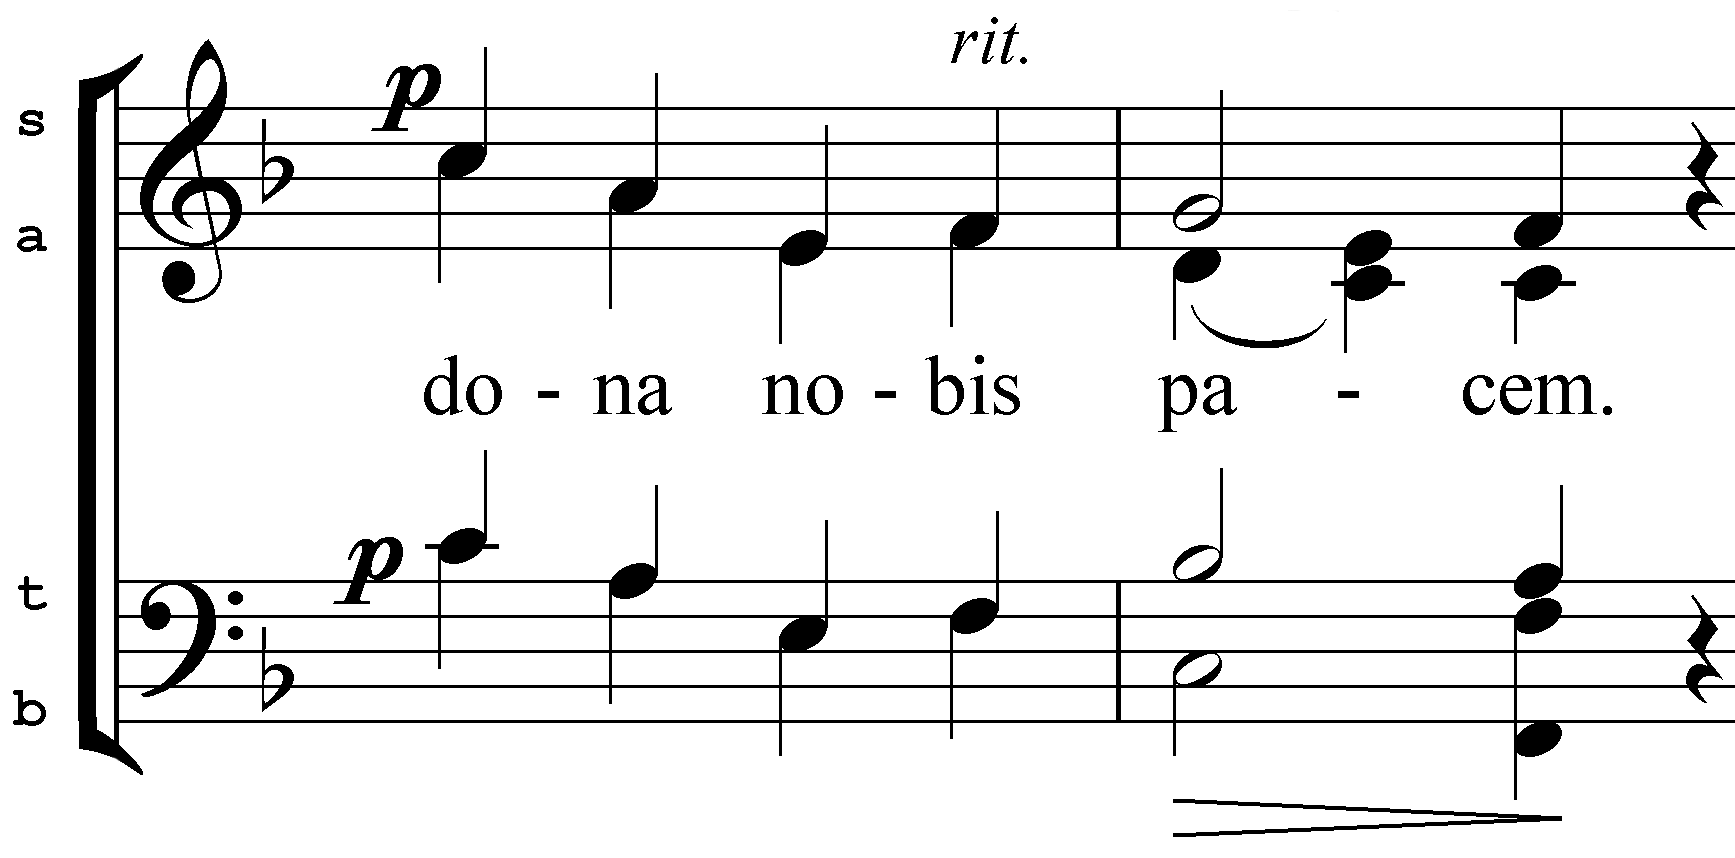
\includegraphics[width=5.692cm,height=2.972cm]{pictures/zulassungsarbeit-img118.png}

Agnus Dei, Takt 50 – 51, Chor\\
\end{supertabular}
\end{flushleft}
\subparagraph{Kyrie}
Besonders dem geschickt gewählten Soggetto ist es zu verdanken, dass das
Kyrie zu den besten Stücken in August Högns kompositorischem Schaffen
zählt. Das Soggetto verleiht dem Stück einerseits einen schwingenden
2er-Puls. Andererseits eignet sich das Soggetto sehr gut zur
imitatorischen Verarbeitung. Es lässt sich taktweise sequenzieren und
auf verschiedene Stimmen aufteilen (Takt 9 – 10 und 17 – 20), wodurch
Fugati entstehen, die auf satztechnischer Ebene auflockern. Von
Soggetto werden weitere Motive, wie zum Beispiel das chromatische
Überleitungsmotiv abgeleitet (c-cis-d: Takt 16 – 17, 11 – 12, 21 – 22,
48 – 49). Dieses Motiv, das sich auf den kleinen Sekundschritt vom
dritten auf den vierten Ton des Soggettos bezieht, trägt zur gemäßigten
Chromatik und harmonischen Farbigkeit des Kyries bei.

Die Textvorlage legt vielen Kyrie-Vertonungen einen dreiteiligen Aufbau
nahe. Zwischen zwei „Kyrie-eleison“-Abschnitten steht ein
„Christe-eleison“-Abschnitt, der sich meistens strukturell von den
beiden Kyrie-Abschnitten abhebt. Dies ist auch bei Högns Komposition
der Fall.

Der erste Kyrie-Abschnitt (Takt 9 – 25) bildet die großformale
dreiteilige Gliederung des ganzen Kyries in einer kleineren Dimension
ab. Anhand der Satztechnik lässt sich der erste Kyrie-Abschnitt in
weitere drei Einheiten unterteilen. Zwei polyphone Einheiten (Takt 9 –
11 und 16 – 24) umgeben eine homophone Einheit (Takt 11 – 15). Auch
harmonisch ist der erste Kyrie-Abschnitt in Analogie zur dreiteiligen
Form des ganzen Kyries angelegt. Die Kyrie-Abschnitte stehen in F-Dur,
der Christe-Abschnitt in B-Dur. Die Ausweichung nach B-Dur (Takt 12 –
18) in der Mitte des ersten Kyrie-Abschnitts, der in F-Dur beginnt und
endet, erinnert an den Christe-Abschnitt in B-Dur des ganzen Kyries,
der von den Kyrie-Abschnitten in F-Dur umgeben ist.

Ein Gegensatz im Aufbau des Christe-Abschnitts (Takt 25 – 40) zu den
zwei Kyrie-Abschnitten wird allein dadurch erreicht, dass dem
Christe-Abschnitt ein Motiv zugrunde liegt, das wenig Ähnlichkeit mit
dem Soggetto aufweist. Das Motiv des Christe-Abschnitts hat im
Gegensatz zum Soggetto einen ungleichmäßigen Rhythmus und eine aufwärts
gerichtete Melodiebewegung. Auch die satztechnische Weiterverarbeitung
des Motivs des Christe-Abschnitt unterscheidet sich zur Verarbeitung
des Soggettos in den Kyrie-Abschnitten. Nur in zwei Takten (Takt 25 –
26) wird das Motiv des Christe-Abschnitts imitatorisch behandelt. Die
dominierende Satztechnick im Christe-Abschnitt ist die Homophonie.

\begin{center}
\begin{minipage}{4.394cm}
\begin{flushleft}
\tablefirsthead{}
\tablehead{}
\tabletail{}
\tablelasttail{}
\begin{supertabular}{m{4.1940002cm}}

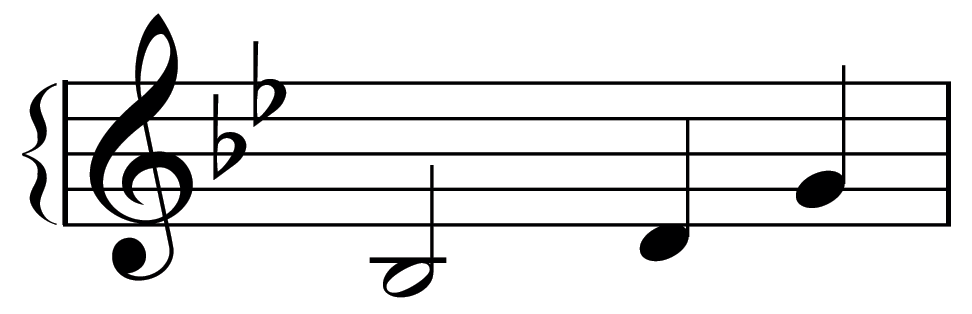
\includegraphics[width=4.011cm,height=1.378cm]{pictures/zulassungsarbeit-img119.png}
\begin{figure}
\img{}
\caption{}
\end{figure}
Motiv des Christe-Abschnitts\\
\end{supertabular}
\end{flushleft}
\end{minipage}
\end{center}
Im zweiten Kyrie-Abschnitt (Takt 41 – 56) werden die ersten 7 Takte des
ersten Kyrie-Abschnitts exakt wiederholt, dann aber schließt sich nur
wenig durch das chromatische Überleitungsmotiv vermittelt eine neue
Einheit (Takt 49 – 55) an, die auf motivischer Ebene scheinbar nur
wenig Ähnlichkeit mit den vorhergehenden Takten hat. Ein Blick in die
Orgelstimme der Takte 49 – 50 verrät, dass Högn auch hier das Soggetto
verwendet, das er aber in den Achtel-Noten der Orgel auflöst. Vor allem
die Achtelbewegung in der Orgel und die Punktierung im Chor tragen dazu
bei, dass das Kyrie in den Takten 49 – 50 seinen Höhepunkt erreicht.
Indem Högn in den Takten 51 – 55 ähnlich frei wie im
Instrumentalvorspiel das Soggetto verarbeitet und viele neue melodische
Momente daraus gewinnt, beruhigt sich der aufgeregte Charakter des
Höhepunkts (Takt 49 – 50) bald und kommt im Nachspiel der Instrumente
(Takt 56 – 60) ganz zur Ruhe.

\subparagraph{Gloria und Credo}
Die Fülle an zu vertonenden Texten fordert im Gloria und Credo eine ganz
andere kompositorische Herangehensweise als bei den Messteilen, die
wesentlich weniger Text als Grundlage haben. Es ist im Gloria und Credo
natürlich weitaus schwieriger als in den Messteilen mit weniger Text
den thematischen Zusammenhalt von Anfang bis zum Ende eines Messteils
aufrecht zu halten und gleichzeitig den musikalischen Ausdruck der
einzelnen Textaussage anzupassen. Högn setzte im Gloria und Credo des
„Josephi“-Messe deutliche Reprisen und erreichte somit einen gewissen
thematischen Zusammenhalt. So entspricht der Beginn des
Quoniam-Abschnitt im Gloria (Takt 53 – 57) und der Beginn des
Et-unam-Sanctam-Abschnitt im Credo (Takt 111 – 116) dem Anfang der
entsprechenden Messteile. Weit mehr als auf einheitliches thematisches
Erscheinungsbild legt Högn Wert auf die musikalische Umsetzung der
Aussagen der einzelnen Textpassagen. In kleinen musikalischen
Einheiten, die sich untereinander durch Tonart, Taktart, Tempo und
Motivik stark unterscheiden können, passt er den Ausdruck ganz der
Aussage des entsprechenden Textes an. Eine derartige „Mosaik-Technik“
setzte Högn zur Vertonung des Glorias und Credos in allen seinen Messen
ein, doch in der „Josephi“-Messe kommt diese Technik „verschärft“ zu
Einsatz. Eine erhöhte Anzahl an Einheiten und damit auch kleinerer
Einheiten deutet die Anzahl der Tempowechsel im Gloria und Credo an.
Sind es in der „Laurentius“-Messe op. 14, seiner ersten Messe, 2
beziehungsweise 3 Tempowechsel, treten im Gloria und Credo der
„Josephi“-Messe 5 beziehungsweise 8 Tempowechsel auf. Auch
unterscheiden sich die einzelnen Einheiten sowohl im musikalischen
Aufbau als auch im Ausdruck mehr als in früheren Werken voneinander.
Ein sehr abrupter Ausdruckswechsel ist vom Et-incarnatus-Abschnitt
(Takt 45 – 56) zum anschließenden Crucifixus-Abschnitt (Takt 57 – 66)
des Credos festzustellen. Auf den im ruhigen, volkstümlichen Ton
gehaltenen Et-incarnatus-Abschnitt folgt plötzlich der scharfe,
verminderte Septakkorde verwendende Crucifixus-Abschnitt.

\begin{center}
\tablefirsthead{}
\tablehead{}
\tabletail{}
\tablelasttail{}
\begin{supertabular}{m{13.070001cm}}

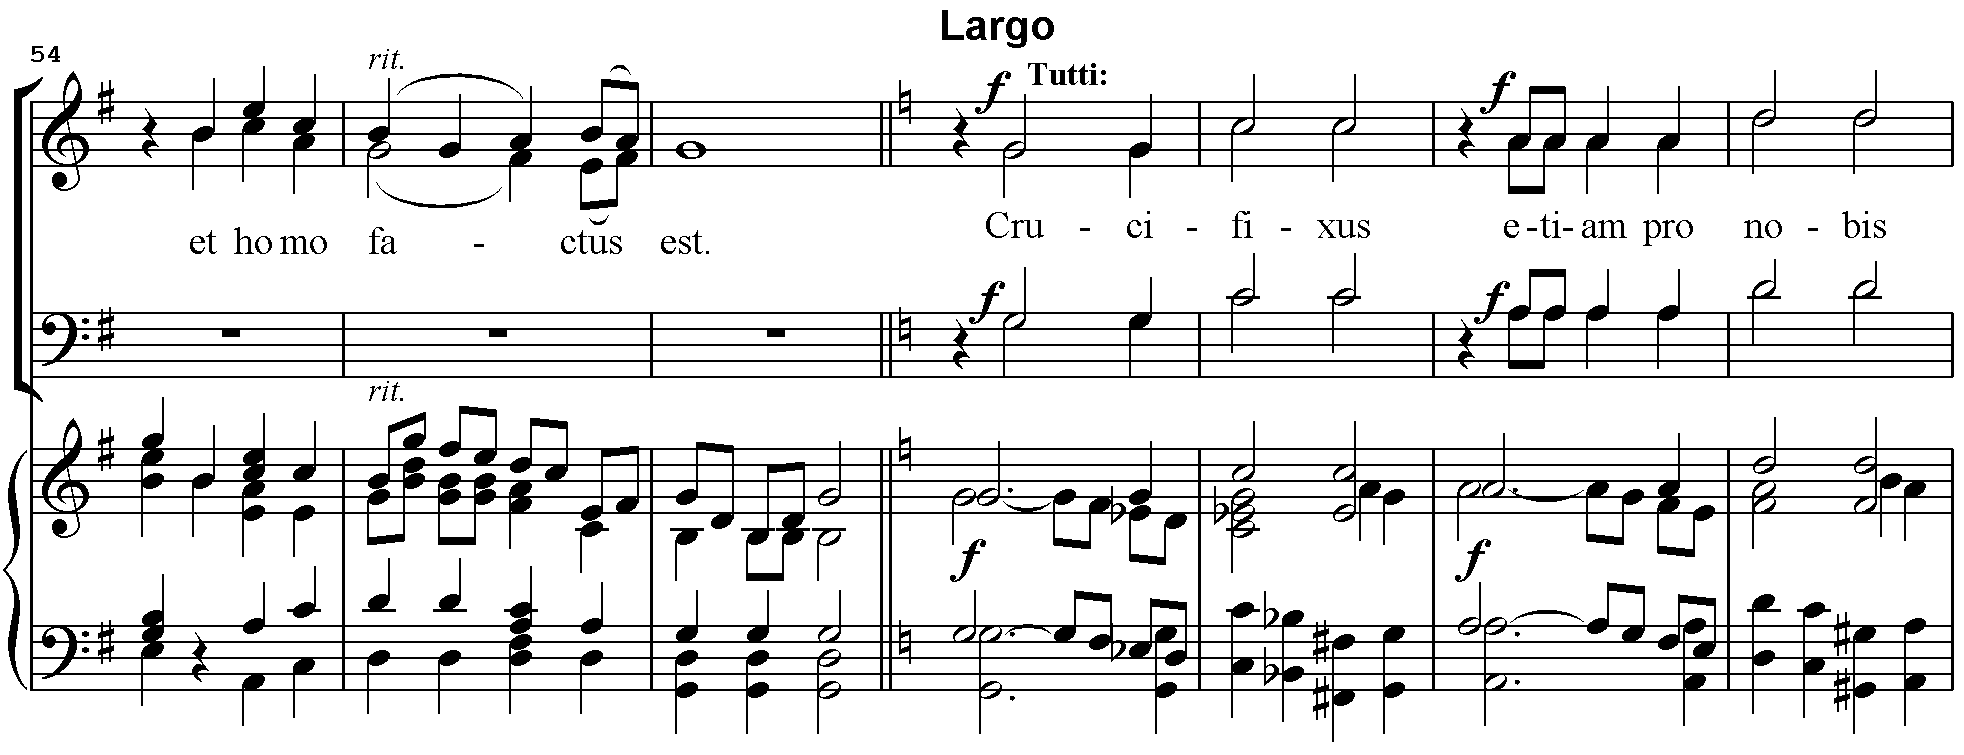
\includegraphics[width=12.887cm,height=4.953cm]{pictures/zulassungsarbeit-img120.png}
\begin{figure}
\img{}
\caption{}
\end{figure}
Credo, Takt 54 – 60, Übergang von dem
Et-incarnatus-Abschnitt zum Crucifixus-Abschnitt, Chor und Orgel

\\
\end{supertabular}
\end{center}
\subparagraph{Sanctus}
Im Sanctus verarbeitet Högn das Soggetto nicht wie im Kyrie
imitatorisch, sondern in einer Art „Collagentechnik.“ Das Soggetto wird
in den Takten 3 und 5 vom Chor in Unisono gesungen. Da die Blechbläser
in den Takten 3 und 5 pausieren, bleiben diese Choreinsätze dem
leichten und schwungvollen Charakter des Kyries treu und wirken wie
eine ferne Reminiszenz an das Kyrie. Umgeben werden diese Choreinsätze
von wuchtigen Vor- und Zwischenspielen aller Instrumente. Die Chor- und
Instrumentaleinsätze wirken auch deshalb so „ineinander geschnitten“,
weil Takte, in denen nur die Instrumente spielen, zum Soggetto
gegensätzliches motivisches Material aufweisen. Dieses Wechselspiel
zwischen Instrumenten und Chor in den Takten 1 – 6 erinnert hier mehr
an eine aus Vorder- und Nachsatz bestehende Periode der Wiener Klassik
als an eine kontrapunktische Form des Cäcilianismus.

\begin{center}
\tablefirsthead{}
\tablehead{}
\tabletail{}
\tablelasttail{}
\begin{supertabular}{m{11.689cm}}
\subparagraph[]{  [Warning: Image ignored]
% Unhandled or unsupported graphics:
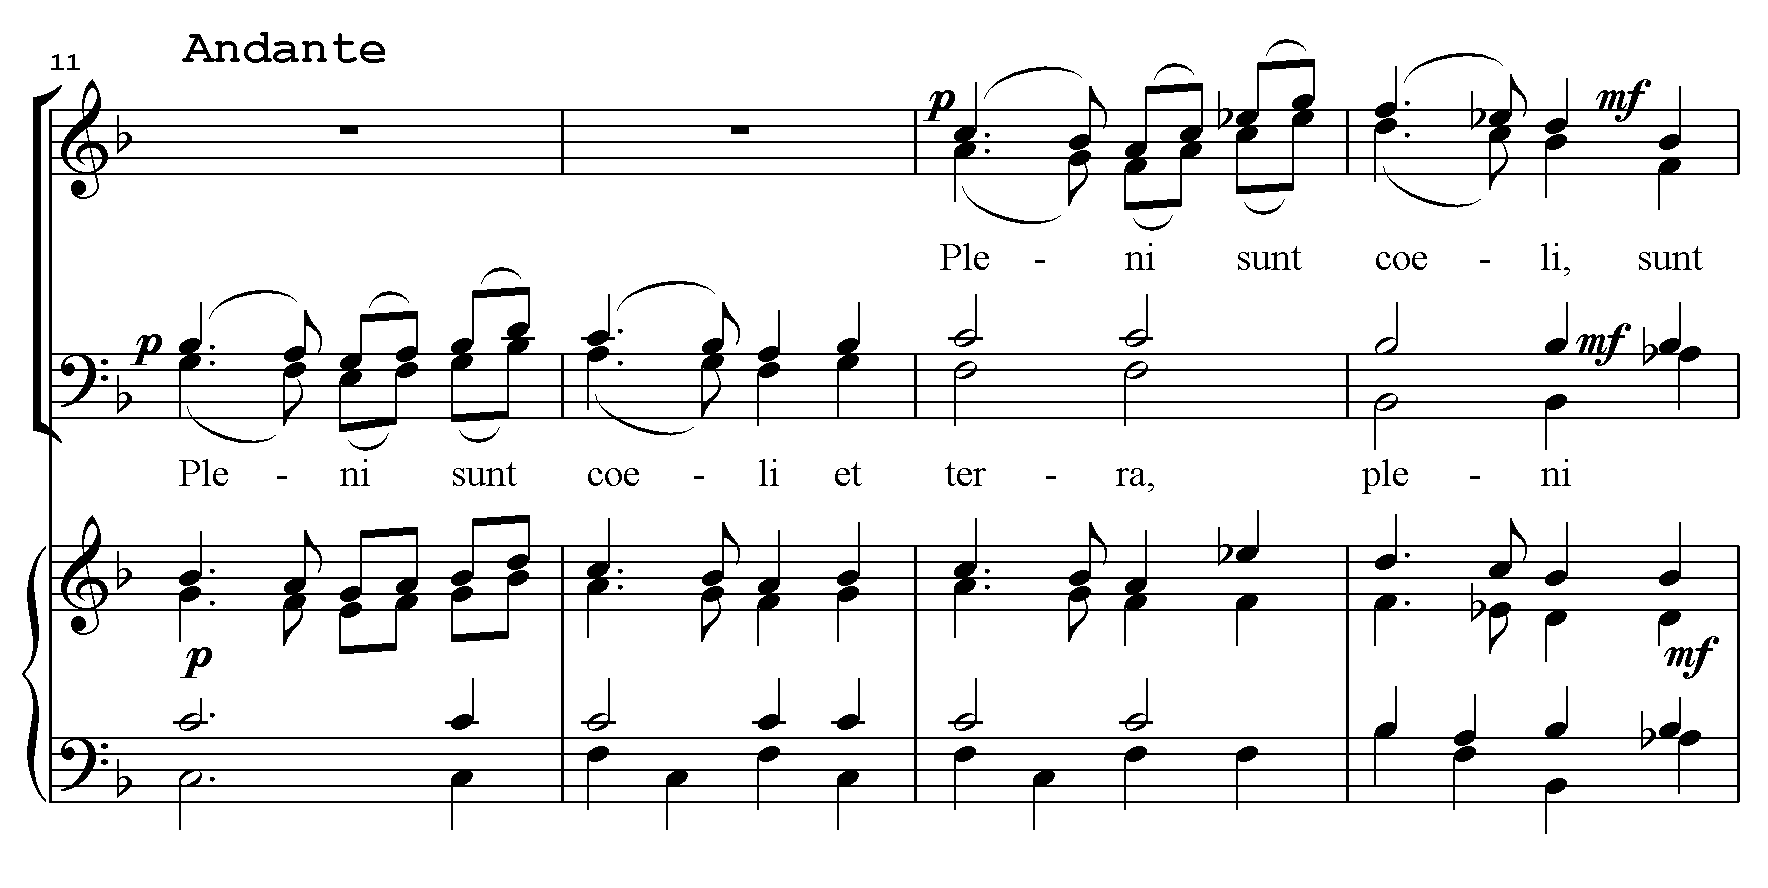
\includegraphics[width=11.506cm,height=5.355cm]{pictures/zulassungsarbeit-img121.png}
 }
Sanctus, Takt 11 – 14\\
\begin{figure}
\img{}
\caption{}
\end{figure}
\end{supertabular}
\end{center}
Der Anfang des „Pleni sunt coeli“ ist ein Beispiel für die Vermischung
von cäcilianischen mit folkloristischen Stilelementen. Unter die
zugegebenermaßen sehr einfache Imitation zwischen Männer- und
Frauenstimmen in den Takten 11 – 14 setzt Högn in der Orgel einen
Wechselbass, der genau so einem Marsch oder einer Polka aus der
Volksmusik entnommen sein könnte.

\subparagraph{Benedictus}
Im Benedictus kommt das Soggetto als einziger Messteil der
„Josephi“-Messe nicht vor. Der Einsatz von Soggetti und die
imitatorische Verarbeitung der Soggetti, wie etwa im Kyrie der
„Josephi“-Messe, ist ein Stilelement des Cäcilianismus. Typisch
cäcilianische Messen vertonen das Benedictus meist in einem Fugato mit
Stimmeinsätzen von oben nach unten, so zum Beispiel die
„Laurentius“-Messe von Högn. In seiner Anlage als Sololied für
Sopransolo mit Chor und Orgelbegleitung ist das Benedictus der
„Josephi“-Messe ausschließlich homophon gesetzt. Das Benedictus ist
deshalb der Messteil, in dem sich Högn vom cäcilianischen Kirchenstil
am weitesten entfernt.

\begin{flushleft}
\tablefirsthead{}
\tablehead{}
\tabletail{}
\tablelasttail{}
\begin{supertabular}{m{10.528cm}}

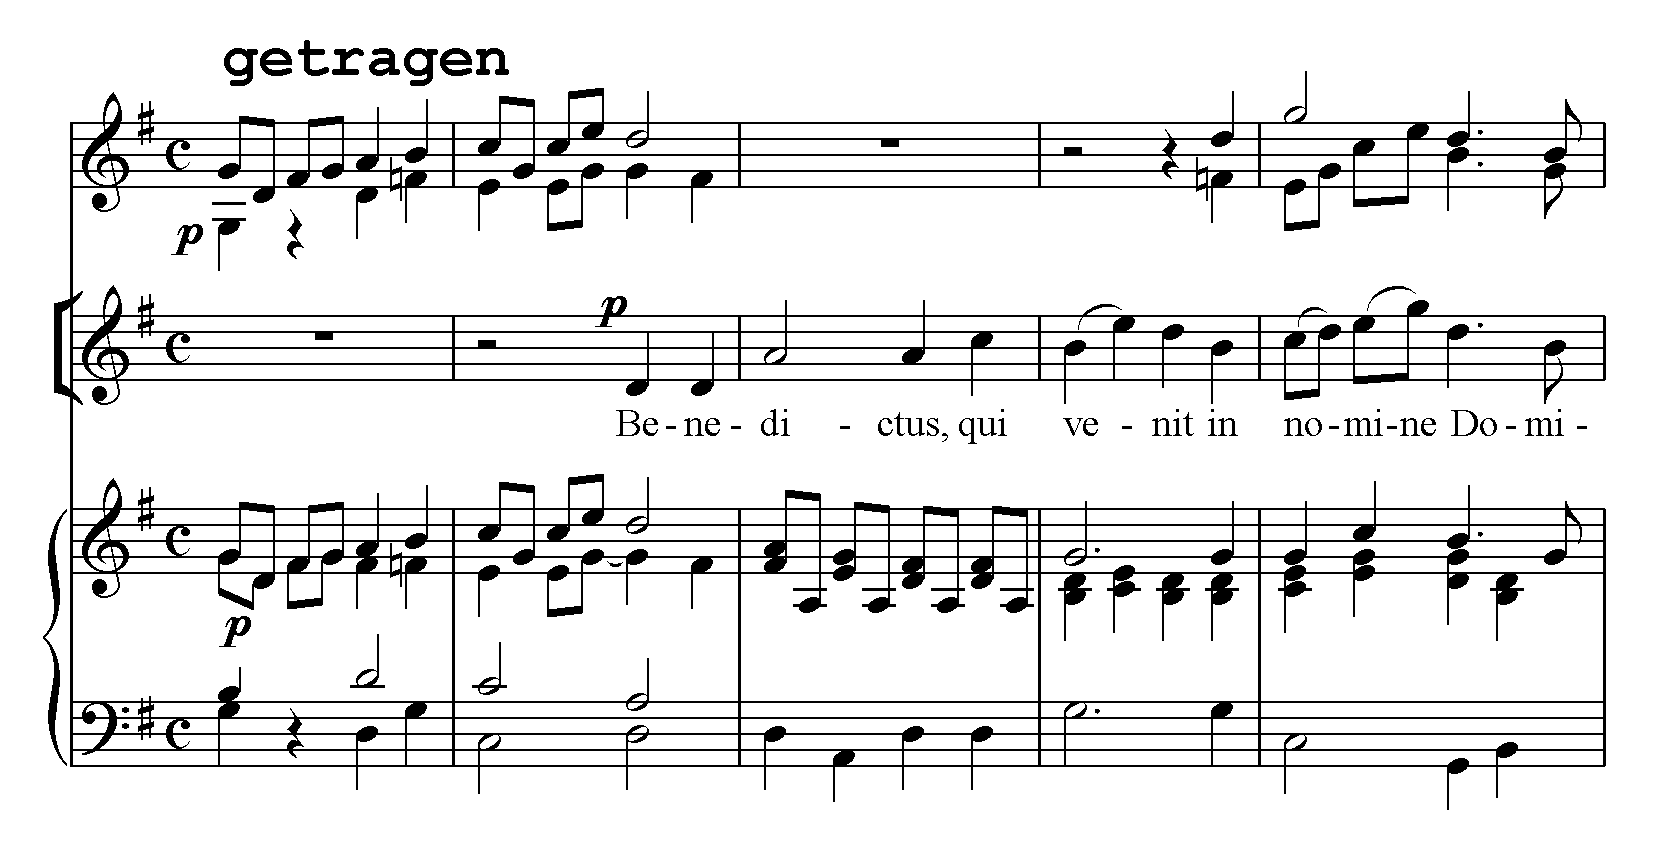
\includegraphics[width=10.345cm,height=5.313cm]{pictures/zulassungsarbeit-img122.png}
\begin{figure}
\img{}
\caption{}
\end{figure}
Benedictus, Takt 1 – 5, Violinen,
Sopran-Solo, Orgel\\
\end{supertabular}
\end{flushleft}
\clearpage\subparagraph{Agnus Dei}
Obwohl Högn das Soggetto zu Beginn des Agnus Dei im Orgelvorspiel nur
wenig verändert, erscheint es hier in einer vollkommen anderen Sphäre.
Die Molleintrübung, der vorangestellte Auftakt und der beschleunigte
Melodiefluss in Achtelbewegung beleuchten das Soggetto von einer
anderen Seite aus. Dabei entsteht ein äußerst reizvolles Thema im
Orgelvorspiel, dass einen willkommenen Gegenpol zum sonst in der Messe
vorherrschen Dur und zu der dominierenden Viertelbewegung darstellt.
Leider wird bereits in Takt 5 mit den einsetzenden Bass-Solo die
Achtelbewegung und in Takt 10 beim Choreinsatz das Moll verlassen und
so nicht nur zur „gewöhnlichen“ Tonsprache der Messe zurückgegangen,
sondern auch thematisch ein Bruch erzeugt. Das Agnus Dei der
„Josephi“-Messe setzt sich ähnlich wie das Gloria und Credo aus
aneinander gereihten Einzelbausteinen zusammen.

\begin{center}
\tablefirsthead{}
\tablehead{}
\tabletail{}
\tablelasttail{}
\begin{supertabular}{m{12.107cm}}

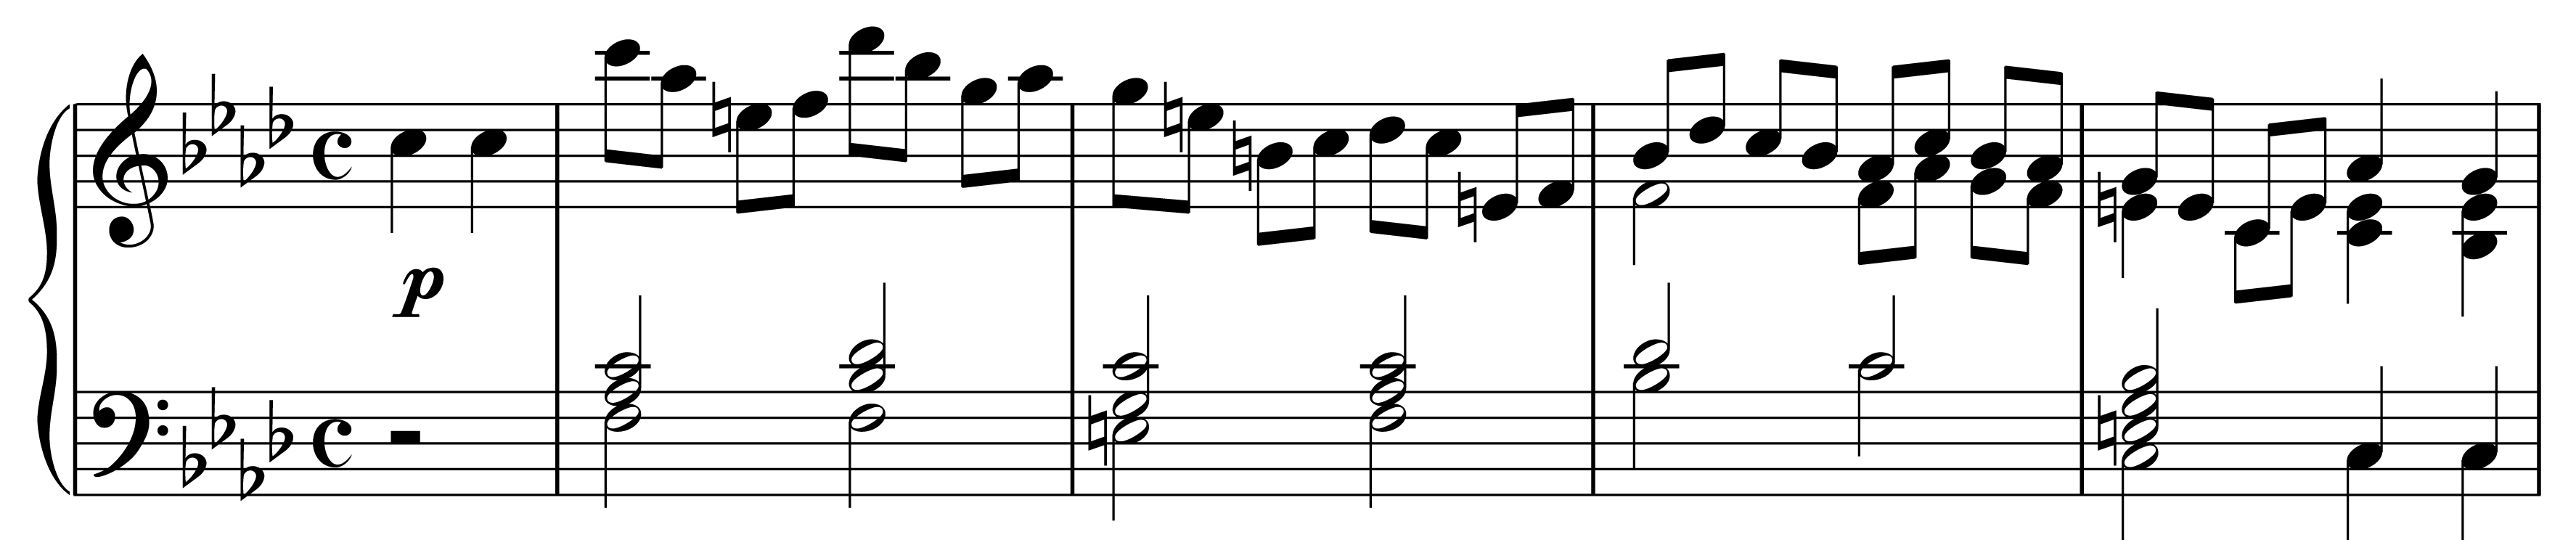
\includegraphics[width=11.924cm,height=2.489cm]{pictures/zulassungsarbeit-img123.png}
\begin{figure}
\img{}
\caption{}
\end{figure}
Agnus Dei, Takt 1 – 5, Orgel\\
\end{supertabular}
\end{center}
Es nehmen weder die Zwischenspiele der Orgel (Takt 14 – 16 und 29 – 33)
noch die Abschnitte mit Chorbeteilung auf das aus dem Soggetto
gesponnene Eingangsthema Bezug. Nur das Soggetto (Takt 2 -3, 6, 33 –
34) sorgt im Agnus Dei für den thematischen Zusammenhalt. Es sind vor
allem die schönen Einzelmomente, wie die miserere-nobis-Vertonung in
den Takten 22 – 28, die den besonderen Reiz des Agnus Deis ausmachen.
Hier gelingt es Högn einen Spannungsbogen vom Unisono der Männerstimmen
(Takt 22 – 23) über die Erweiterung des Tonraums durch Einsatz der
Frauenstimmen (Takt 24 – 25) zum Höhepunkt im Takt 26 und den
langsamen, sequenzartigen Spannungsabbau im Chor-a-cappela (Takt 26 –
29) zu ziehen.

Im Dona-nobis-Abschnitt (Takt 40 – 53) wird wie bei vielen
Messkompositionen üblich auch in der „Josephi“-Messe das Kyrie
thematisch wieder aufgenommen. Die ersten drei Takte des „Dona nobis“
sind deshalb abgesehen von den Violinstimmen identisch mit dem
Choreinsatz des Kyrie. In Takt 43 führt Högn ein neues Motiv ein,
behandelt dies aber nur kurz imitatorisch, ehe er in Takt 48 einen Takt
aus dem Orgelvorspiel zu Beginn des Kyrie zitiert und in Takt 50 das
Soggetto in seiner Urform von Chor unisono gesungen zum letzten Mal
erklingen lässt. Das Ende der „Josephi“-Messe ist auf ein langsames
Verklingen hin komponiert, zwei F-Dur-Akkorde in Terzlage und im Forte
beenden die Messe aber schließlich ebenso abrupt wie fulminant und
nicht ohne Pathos.